\graphicspath{ {LiveAudioWatermarking/Images/} }
\chapter{Introduction}
The goal of this chapter is to introduce the main technologies that are used to build a modern microphone: MEMS and ECM. 


In the next chapter the watermarking procedure will be described in detail and how such technique helped to implement the use case of the project. \newline
Chapter 3 describes the state of the art of modern day attacks and then in the last chapters the implementation and the results of the project will be discussed.
\section{State of the Art: MEMS and ECM}
\subsection{MEMS Microphone}
MEMS (Micro-Electro-Mechanical System) Microphones use a MEMS component placed on a printed circuit board (PCB) and protected with a mechanical cover. A small hole is fabricated in the case to allow sound into the microphone and is either designated as top-ported if the hole is in the top cover or bottom-ported if the hole is in the PCB. The MEMS component is often designed with a mechanical diaphragm and mounting structure created on a semiconductor die.
\subsection{How it works}
The MEMS diaphragm forms a capacitor and sound pressure waves cause movement of the diaphragm. MEMS microphones typically contain a second semiconductor die which functions as an audio preamplifier, converting the changing capacitance of the MEMS to an electrical signal. The output of the audio preamplifier is provided to the user if an analog output signal is desired. If a digital output signal is desired, then an analog-to-digital converter (ADC) is included on the same die as the audio preamplifier. A common format used for the digital encoding in MEMS microphones is pulse density modulation (PDM), which allows for communication with only a clock and a single data line. Decoding of the digital signal at the receiver is simplified due to the single bit encoding of the data. Digital I²S outputs are a third option that include an internal decimation filter, which allows for processing to be completed in the microphone itself. This means the microphone can connect directly to a digital signal processor (DSP) or microcontroller, eliminating the need for an ADC or codec in many applications.
\begin{figure}[H]
    \centering
    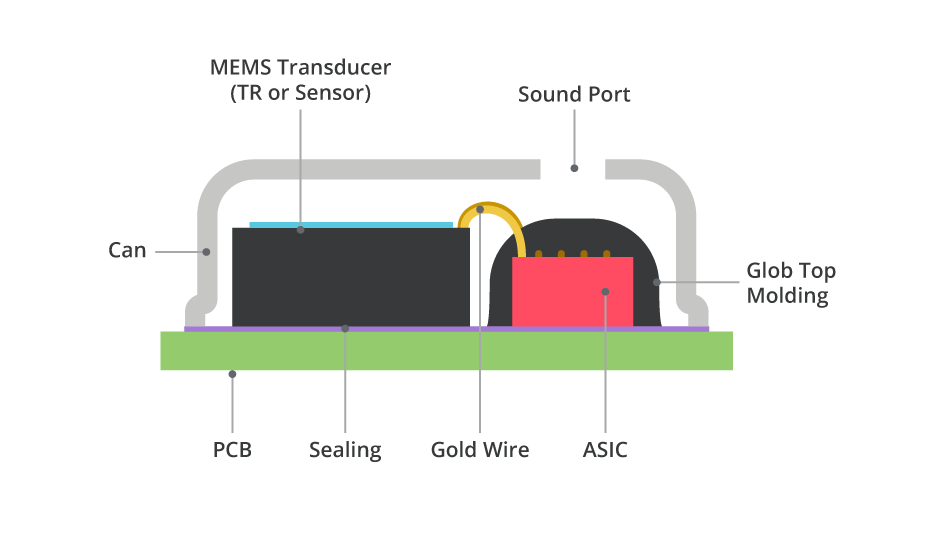
\includegraphics[width=8cm]{LiveAudioWatermarking/images/MEMS.png}
    \caption{: MEMS Structure}
    \label{fig:MEMS}
\end{figure}

\subsection{ECM}
An electret diaphragm (material with a fixed surface charge) is spaced close to a conductive plate, and similar to MEMS microphones, a capacitor is formed with the air gap as the dielectric. Voltage across the capacitor varies as the value of the capacitance changes due to sound pressure waves moving the electret diaphragm, $\Delta$V = Q/ $\Delta$C. The capacitor voltage variations are amplified and buffered by a JFET internal to the microphone housing. The JFET is typically configured in a common-source configuration, while an external load resistor and dc blocking capacitor are used in the external application circuit. \cite{mems}
\break
\begin{figure}[H]
    \centering
    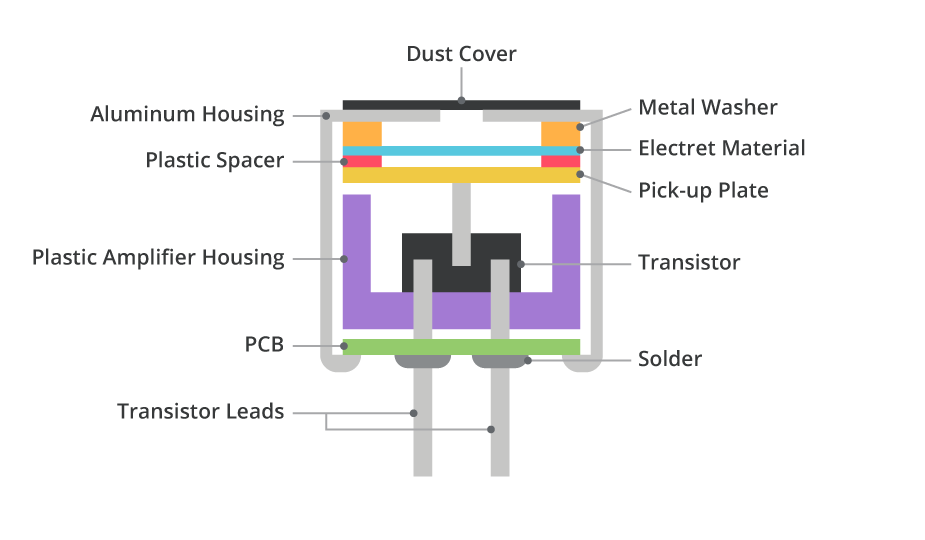
\includegraphics[width=8cm]{LiveAudioWatermarking/images/ECM.png}
    \caption{: ECM Structure}
    \label{fig:ECM}
\end{figure}
\section{Main differences}
Due to their small size, electrical noise immunity, and mechanical robustness, MEMS microphones are becoming increasingly popular. However, this does not mean that they are the de-facto best choice for every application. Many legacy applications may benefit from a simple change or upgrade to their current ECM. Apart from their excellent IP ratings, which allow them to perform well in harsh environments, the intrinsic nature of ECMs also makes them an excellent choice for applications that benefit from noise-canceling or unidirectionality.
\newpage
If the space constraints placed upon a design are particularly acute (such as in smartphones, wearables, hearing aid implants, etc.), or there is likely to be the need to distribute multiple microphones throughout an item of equipment (like in a VR headset for instance) then MEMS may be the better option.
Conversely, if elevated performance or resilience to challenging operating conditions are a priority, then ECM could prove to be the more appropriate route to take. Therefore, professional audio equipment, voice-controlled home assistants, voice recognition systems, and a wide range of other applications will continue to rely on these devices. \cite{compare}





 During the last decade the usage of MEMS in common devices raised significatively (back in 2009 when Apple started to use MEMS microphones for iPhone 4) and since the project focused on such devices like smartphones due to the nature of the attack and the target of the attacks, the solution that has been implemented was on MEMS microphones.
 As shown in Figure 1.3 it is possible to understand why it is much more useful for the purpose of this project to consider MEMS technology rather than the ECM, it is sufficient to consider Average Growth Rate to take into account the rising of the first technology and the falling of the latter.

 
 \begin{figure}[H]
    \centering
    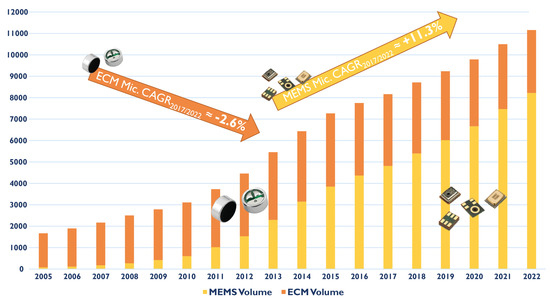
\includegraphics[width=10cm]{LiveAudioWatermarking/images/market.jpg}
    \caption{: Market Evolution}
    \label{fig:market}
\end{figure}

\section{Exploiting Non-Linearity in MEMS microphones}
Even though this effect is not exploited unless very high frequencies (order of 60kHz) are used it is really important to describe one of the core development of this project: the non-linearity of this technology.

Modules inside a microphone are mostly linear systems, in the case of the pre-amplifier with input S:
\[ S_{out} = A_1S\]
Acoustic amplifiers maintain a strong linearity only in the audible frequency range but outside of this range the response exhibits non linearity. Thus, for f $>$ 25kHz, the net recorded $S_{out}$ can be expressed as:
\[S_{out}\Bigg|_{f>25} = \sum_{i=1}^{\infty}A_iS^i=A_1S+A_2S^2+A_3S^3+...\]
With the third and higher terms that are extremely weak and can be ignored.

\newpage
To operate the microphone in its non-linear range, one can play a sound S composed of two tones S$_1$ = 40 and S$_2$ = 50 kHz.
S = $Sin(2\pi40t)+Sin(2\pi50t)$.
After passing through the diaphragm and pre-amplifier of the microphone, the output $S_{out}$ can be modeled as:
\[S_{out}= A_1(S_1 + S_2) + A_2(S_1 + S_2)^2 =\] \[ = A_1[Sin(\omega_1t) + Sin(\omega_2t)] + A_2 [Sin^2(\omega_1t) + Sin^2(\omega_2t) + 2Sin(\omega_1t)Sin(\omega_2t)\]
where $\omega_1$ = 2$\pi$40 and $\omega_2$ = 2$\pi$50.



The first order terms produce frequencies out of the microphone's cutoff, the second order term  instead is a multiplication of signals, resulting in different frequencies for each component such as 2$\omega_1$, 2$\omega_2$, ($\omega_1$ - $\omega_2$) and ($\omega_1$ + $\omega_2$). Mathematically, 
\[ A_2(S_1 + S_2)^2 = 1 - \frac{1}{2}Cos(2\omega_1t) - \frac{1}{2}Cos(2\omega_2t) + Cos((\omega_1 - \omega_2)t) - Cos((\omega_1 + \omega_2)t)\]
With the cutoff frequency at 24kHz, every frequency gets filtered except for the $\omega_1 - \omega_2$ component, that results in a 10kHz tone, this allows a totally inaudible frequency to be recorded by the microphone.
This is the main concept that revolves around this project and some possible future implementations and improvements. \cite{backdoor}




The goal of the project proposed is to show how some high frequency tones can carry some data thanks to Watermarking, anyway if the data can be carried at such high frequency the future improvement can basically carry these information at an even higher frequency thanks to the implementation of an amplifier and work at inaudible frequencies.



 \begin{figure}[H]
    \centering
    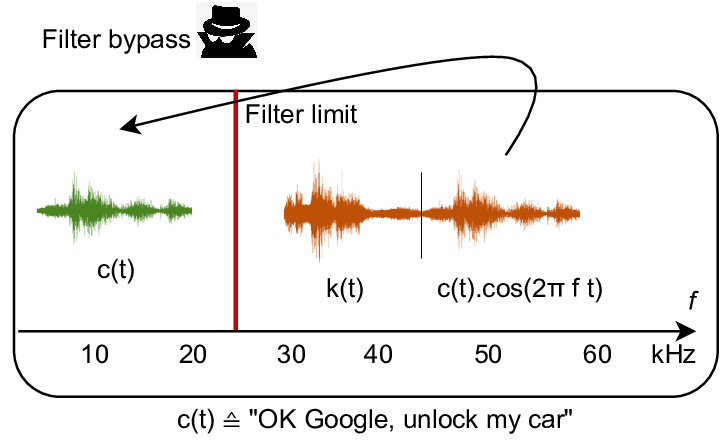
\includegraphics[width=10cm]{LiveAudioWatermarking/images/Bypass.png}
    \caption{: Example of a filter bypass exploiting non linearity}
    \label{fig:market}
\end{figure}